\chapter{概率图模型概述}
\label{chap:pgm-overview}

一台设备发出报警，维修人员需要判断是否停机检查。设备故障造成的过热和传感器失灵都可能触发报警，因此同一条报警记录可以对应不同的内部状态。判断“有故障”之外，还需要估计故障发生的概率，并结合后续温度读数更新判断。故障概率为$0.02$与$0.45$时，即使模型给出同一个分类结果，停机决策所依据的风险也不同。

设备诊断因而需要一个同时描述故障、温度与报警的分布。\term{概率图模型}（probabilistic graphical model, PGM）将这些随机变量画成节点，用图组织局部依赖，再由局部概率函数组成联合分布。可信的局部依赖假设可以减少需要指定的概率，也为复用计算提供依据。本章沿着设备诊断展开：先说明分布保留了哪些预测信息，再建立图与联合分布的关系，最后区分根据证据查询概率和根据数据确定模型这两类任务。

\section{从单值预测到结构化分布}
\label{sec:pgm-overview-distribution-prediction}

以传感器读数$x$预测设备下一时刻的温度时，模型可以返回$\hat y=f(x)$。这种\term{点预测}（point prediction）用一个数值概括输出，分类任务则用一个类别概括输出。它能直接进入后续决策，但单个结果中包含的信息有限，例如一个温度均值没有说明高温状态出现的概率。

保留这些信息的一种方式是给出\term{预测分布}（predictive distribution）$p(y\mid x)$，描述输入固定后各个输出的可能性。离散输出由每种结果的概率表示，连续输出由概率密度表示，落入某个区间的概率通过积分得到。分布可以同时呈现结果的集中位置、分散程度和多个分离的高概率区域。

图~\ref{fig:pgm-overview-predictive-density}用一个人工设定的温度分布说明这种区别。冷却系统有两种可能工况，预测密度分别集中在$40\,^\circ\mathrm{C}$和$80\,^\circ\mathrm{C}$附近，权重各为一半。两种工况的平均温度是$60\,^\circ\mathrm{C}$，恰好落在两个峰之间的低密度区域。保留完整分布能够同时呈现高温和低温工况；用均值或其中一个峰作点预测，则分别丢失峰的位置或另一种工况的信息。

\begin{figure}[htbp]
  \centering
  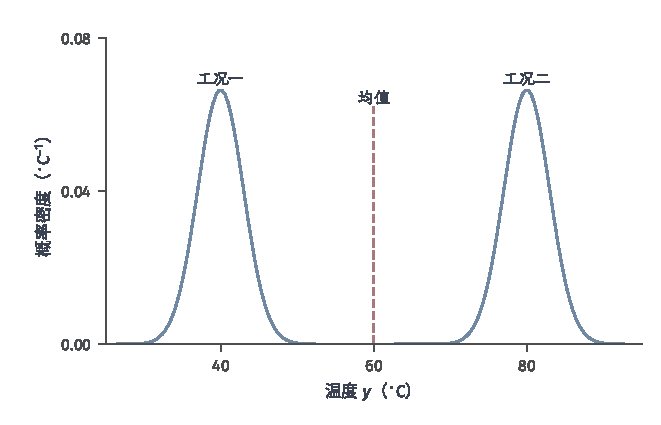
\includegraphics[width=105.412mm]{figures/06-probabilistic-graphical-models/01-representation/matplotlib/pgm-overview-predictive-density/figure.pdf}
  \caption{温度预测中的双峰分布与均值。实线为两个等权高斯密度的混合，每个分量的标准差为$3\,^\circ\mathrm{C}$；虚线标出均值$60\,^\circ\mathrm{C}$。两种工况集中在均值两侧，因而均值这一点预测省略了高概率区域的位置。图中分布为教学设定。}
  \label{fig:pgm-overview-predictive-density}
\end{figure}

预测分布也可以用来产生点预测。设备控制需要一个温度设定值时，可以从分布中选择均值；判断最可能工况时，可以选择概率最大的结果；停机决策则需要把可能的损失一并考虑。分布保留输出的不确定性，具体任务决定怎样将这些信息转化为数值、类别或行动。

当设备包含多个相互影响的部件时，预测还需要联合描述它们的状态。$d$个二值变量共有$2^d$种状态组合，直接指定完整联合表需要$2^d-1$个自由参数。变量数量增加会使数据分散在更多组合中，边缘概率的计算也可能涉及大量状态的汇总。利用局部依赖组织联合分布，正是为了在假设允许的范围内减少参数和计算。

故障与报警之间的联系必须保留，因而把所有变量设为相互独立会损失诊断所需的信息。局部简化可以更有针对性：假设报警只直接依赖过热和传感器失灵，那么给定这两个状态后，故障状态便不再改变报警的局部概率。这种“给定哪些状态后，另一个状态不再提供额外信息”的关系由条件独立表达，并由图结构记录。

\section{图模型上的表示}
\label{sec:pgm-overview-representation}
\label{sec:pgm-overview-basic-concepts}

为具体描述设备诊断，引入四个二值随机变量：故障$F$、过热$H$、报警$A$和传感器失灵$S$，取值$1$表示相应事件发生，取值$0$表示未发生。小写字母表示这些变量的取值，因此$p(f,h,a,s)$给出四个状态同时成立的联合概率。

有向图、因子图、团树和缺失数据图分别突出变量依赖、乘积分解、消息传递和观测状态，图~\ref{fig:pgm-overview-visual-conventions}汇总它们使用的视觉符号。节点的外形和填色区分变量、局部函数与给定量，连线的含义则由图中所描述的对象决定。尤其是虚线，可能表示辅助对应、证据读入或分隔边界，其具体作用会在相应图内或图注中说明。
\begin{figure*}[htbp]
  \centering
  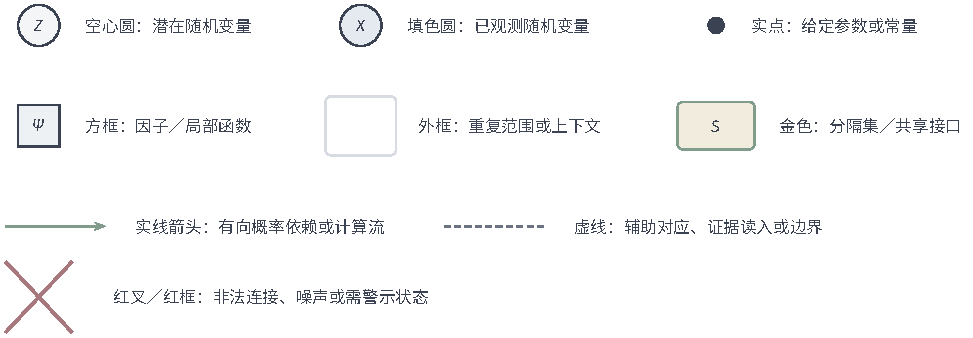
\includegraphics[width=164.747mm]{figures/06-probabilistic-graphical-models/01-representation/tikz/pgm-overview-visual-conventions/figure.pdf}
  \caption{本部分图示的默认视觉符号。空心、填色和实点区分潜变量、观测变量与给定量；方框表示局部因子，浅色填充与绿色轮廓强调团树分隔集或共享接口，红色标出非法或需警示的对象。实线箭头可以表示概率分解或计算流，虚线用于辅助表达，具体含义由各图的标注和图注确定。}
  \label{fig:pgm-overview-visual-conventions}
\end{figure*}

报警记录只给出$A$，而故障判断涉及$F$；过热和传感器状态仍然未知。先对$H,S$的所有取值求和，得到$F,A$的边缘分布，再固定报警取值并归一化，就得到所需条件分布：
\begin{equation}
  p(f,a)=\sum_{h,s}p(f,h,a,s),
  \qquad
  p(f\mid a)=\frac{p(f,a)}{p(a)},\quad p(a)>0.
  \label{eq:pgm-overview-marginal-conditional}
\end{equation}
第一式汇总了每一种未知状态组合，第二式以证据概率$p(a)$为分母，使给定报警后各个故障取值的概率之和为$1$。连续变量通过相应积分消去。条件分布的概率运算参见\BookSectionRef{sec:rv-conditional-distribution}{第一卷“数学准备”的条件分布小节}。

上述局部假设用条件独立记号$X\perp Y\mid Z$表达：给定$Z$以后，$Y$不再为$X$的分布提供额外信息。对于一般随机变量，相关条件分布等式按$Z$的分布几乎处处成立。其概率含义参见\BookSectionRef{sec:probability-moments-independence}{第一卷“数学准备”的独立关系小节}；这里关注这些约束怎样通过图组织起来，并用于简化联合表示和推断。

从完整联合分布出发，链式法则给出$p(f,s,h,a)=p(f)p(s\mid f)p(h\mid f,s)p(a\mid f,s,h)$。右侧仍保留每个变量之前的全部条件，因此所需参数与完整联合表相同。条件独立假设进一步确定哪些条件可以省去，才产生较小的局部函数。

设备模型采用如下假设：故障$F$与传感器失灵$S$独立，过热$H$只直接依赖故障，报警$A$只直接依赖过热和传感器状态。将这些假设代入链式分解，可以分别简化传感器、过热与报警的条件，得到
\begin{equation}
  p(f,h,a,s)=p(f)p(s)p(h\mid f)p(a\mid h,s).
  \label{eq:pgm-overview-device-joint}
\end{equation}
每个局部条件分布对其输出变量归一化，便能保证上述乘积定义一个完整联合分布。二值根变量$F,S$各需一个参数；$H$在$F$的两个取值下各需一个参数；$A$在$(H,S)$的四种组合下各需一个参数。总计$8$个自由参数，而完整联合表需要$15$个；节省来自模型所采用的独立性假设。

式~\eqref{eq:pgm-overview-device-joint}还可以画成图~\ref{fig:pgm-overview-device-graph}：每个节点对应一个随机变量，进入该节点的箭头来自它的局部条件分布所依赖的变量。例如，$H\to A\leftarrow S$把$p(a\mid h,s)$的两个条件显式画出。这些箭头首先具有概率分解的含义；赋予它们因果含义还需要额外的建模假设。

\begin{figure}[htbp]
  \centering
  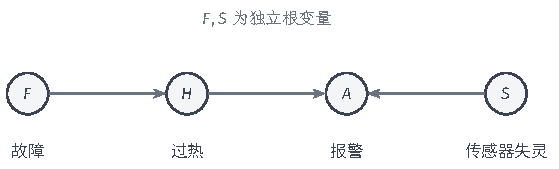
\includegraphics[width=94.590mm]{figures/06-probabilistic-graphical-models/01-representation/tikz/pgm-overview-device-graph/figure.pdf}
  \caption{设备诊断的有向表示。节点表示随机变量，进入节点的箭头指定其局部条件分布所依赖的变量，例如$H\to A\leftarrow S$对应$p(a\mid h,s)$。这里的箭头记录概率分解，因果解释需要另行给出假设。}
  \label{fig:pgm-overview-device-graph}
\end{figure}

图和局部函数共同确定模型。设备图规定报警概率以$H,S$为条件，局部表$p(a\mid h,s)$则给出每种状态组合下报警的具体概率。同一个图可以配上不同的数值表，从而给出不同的诊断结果；图结构组织依赖，局部函数决定这些依赖的数值。

设备模型属于\term{有向图模型}（directed graphical model），它由图中的父子方向组织局部条件分布的乘积。第~\ref{chap:pgm-directed}章将进一步说明这种分解与图上的条件独立关系怎样对应。

邻近部件之间的对称相互作用则可以用\term{无向图模型}（undirected graphical model）表示。它把局部关系写为非负函数$\psi_c(\bm x_c)\geq0$，并将乘积归一化，得到$p(\bm x)=Z^{-1}\prod_c\psi_c(\bm x_c)$，其中$Z=\sum_{\bm x}\prod_c\psi_c(\bm x_c)$，连续情形用积分。局部势函数描述配置之间的相对权重，全局常数$Z$负责归一化；$0<Z<\infty$时，才得到合法概率分布。第~\ref{chap:pgm-undirected}章将解释无向边、势函数和条件独立之间的关系。

计算局部乘积时，还可以使用\term{因子图}（factor graph）。它将随机变量和局部函数分别画成两类节点，函数涉及哪个变量，就在两者之间连边。设备模型中的$p(a\mid h,s)$因子因而连接$A,H,S$，清楚显示该项参与了哪些变量的计算。

有向模型的条件概率乘积和无向模型的势函数乘积都能转换为因子图。转换保留选定的乘积分解，而原有父子方向需要由函数含义补充说明。因此，因子图主要提供局部计算的组织方式，第~\ref{chap:pgm-representations}章将比较不同表示保留的结构信息。PRML第8章也从概率分解出发介绍这些图表示\scite{bishop2006}。

\section{图模型上的推断与学习}
\label{sec:pgm-overview-inference-learning}

报警记录提出的查询是$p(F=1\mid A=1)$。在图结构和局部概率已知时，根据证据计算这种查询称为\term{概率推断}（probabilistic inference）。过热$H$和传感器状态$S$仍然未知，所以推断要把它们可能处于的每一种状态都纳入后验计算。

为观察计算量如何变化，将诊断范围扩展到更多部件，并设共有$30$个未观测的二值状态，包括$H,S$以及新增的部件或运行状态。将它们统一记为$\bm{Z}=(Z_1,\ldots,Z_{30})$，仍以报警$A=1$为证据、故障$F$为查询目标。后验的分子汇总故障发生时的未知配置，分母汇总故障两种取值下的配置：
\begin{equation}
  p(F=1\mid A=1)
  =
  \frac{
    \displaystyle\sum_{\bm{z}\in\{0,1\}^{30}}
    p(F=1,A=1,\bm{z})
  }{
    \displaystyle\sum_{f\in\{0,1\}}
    \sum_{\bm{z}\in\{0,1\}^{30}}
    p(f,A=1,\bm{z})
  }.
  \label{eq:pgm-overview-expanded-diagnosis}
\end{equation}
直接展开该式时，分子包含$2^{30}$个未观测状态配置，约为$10.7$亿项；分母同时遍历故障的两个取值，包含$2^{31}$个完整配置项，约为$21.5$亿项。这是对状态组合的计数，所需模型参数仍由局部函数决定。

对于一个完整配置$p(f,A=1,\bm{z})$，局部分解允许逐项查表或计算，再将结果相乘。后验却要汇总许多这样的配置，因此主要开销可能来自求和，而非单次乘积评价。若不同配置共享某些局部计算，图结构便可能帮助复用这些结果；复用范围和中间结果大小取决于变量之间的连接方式。

\term{精确推断}（exact inference）重组概率运算，在给定模型下求出原查询的准确答案，其时间和空间开销受问题规模及中间结果大小影响。预算不足以容纳这些中间计算时，可以采用\term{近似推断}（approximate inference），在可承受的时间或空间内估计查询，并分析所引入的误差。第~\ref{chap:pgm-elimination}章至第~\ref{chap:pgm-sampling}章分别讨论这些计算方法及其适用结构。

设备运行记录可以用来确定局部概率的数值。例如，在故障和过热状态均被记录时，故障设备中过热的比例可以用于估计$p(H=1\mid F=1)$。在图结构和局部函数形式给定的前提下估计这些数值，称为\term{参数学习}（parameter learning）。稀有状态只有少量样本时，估计受随机波动影响较大；存在缺失或潜变量时，还需要处理无法直接取得的状态计数。

若设备内部哪些状态应当直接相连也未知，就需要根据数据和领域约束选择图，这称为\term{结构学习}（structure learning）。增加连接可以描述更多依赖，通常也会扩大局部函数并增加估计和推断的开销；减少连接则需要确认相应独立性假设是否适合数据。学习所得的有向结构首先描述概率关系，因果解释仍取决于额外假设和证据。

这两类学习任务确定模型，而推断利用给定模型计算未知状态的概率。含有未观测变量的数据将二者联系起来：参数更新所需的统计量可能依赖潜在状态，于是先用当前模型计算这些状态的后验，再据此更新参数。第~\ref{chap:pgm-parameter-learning}和第~\ref{chap:pgm-structure-learning}章将分别展开参数估计与结构选择。

\section{概率图模型的历史}
\label{sec:pgm-overview-history}

局部相互作用如何组成整体分布，观测如何改变未知状态的概率，未知参数又如何从数据中估计，这些问题推动了概率图模型的发展。图~\ref{fig:pgm-overview-history}将代表工作放在同一条历史线上，以下结合各自处理的计算与建模问题说明它们的联系。

\begin{figure*}[p]
\centering
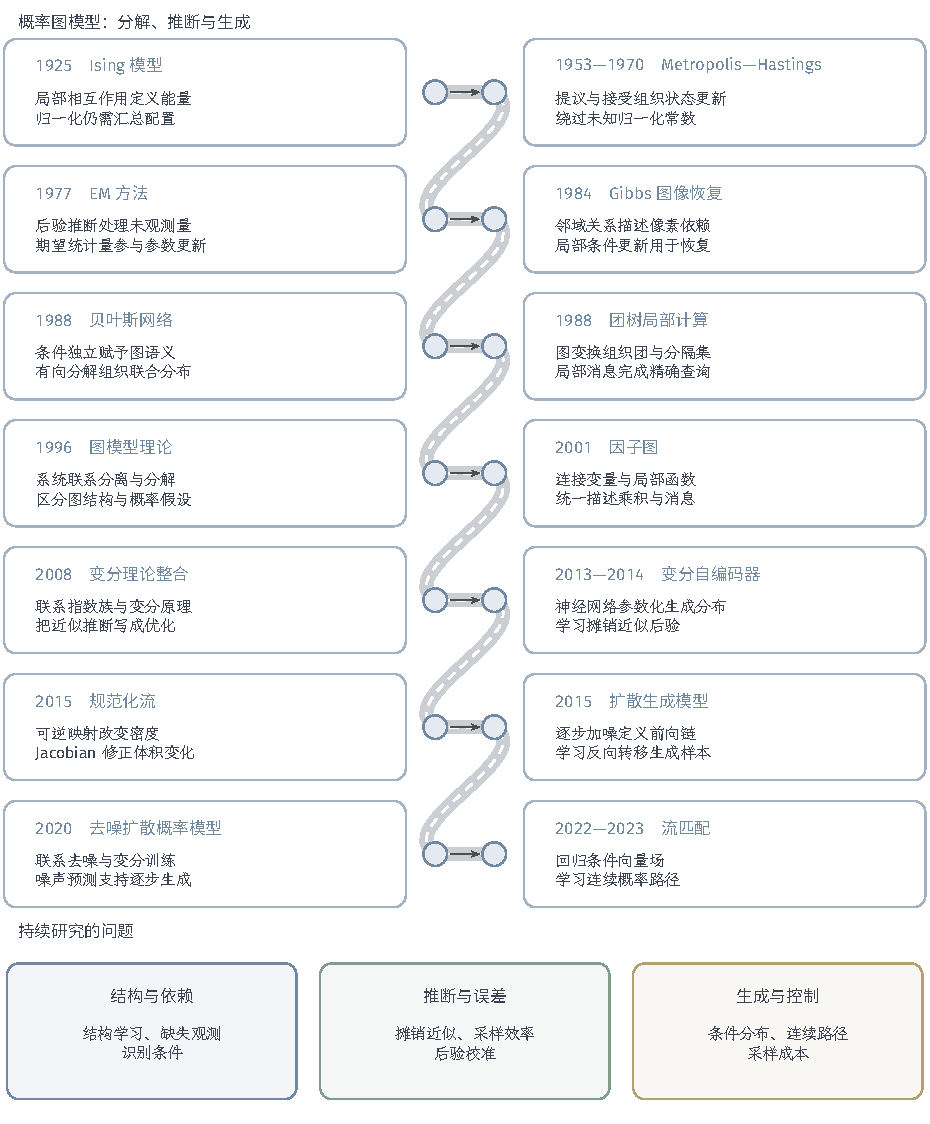
\includegraphics[width=157.406mm]{figures/06-probabilistic-graphical-models/04-models/tikz/pgm-models-history/figure.pdf}
\caption{概率图模型发展的代表工作。局部随机模型组织联合分布，图结构表达独立性，推断与学习算法处理未知状态和参数，神经参数化扩展局部函数与生成路径。2008年标出变分理论的系统整合工作；各年份对应图中所列代表文献，节点间距仅用于排版。}
  \label{fig:pgm-overview-history}
\end{figure*}

\subsection{从局部随机规律到图结构语义}

1925年的Ising模型以相邻自旋的相互作用描述整体配置，是无向局部随机模型的早期代表。每个局部项只涉及少量自旋，而归一化常数与边缘概率仍涉及整体状态的汇总。另一类问题来自数据中的未观测变量：1977年的EM方法利用当前模型推断相关统计量，再让这些统计量参与参数更新\scite{pgm-overview-ising1925,pgm-overview-dempster1977}。

归一化常数难以直接求出时，状态更新提供了另一条计算路线。1953年的Metropolis方法及1970年的Hastings推广通过提议候选状态与决定是否接受，构造随机轨迹；接受比中共同的未知归一化常数可以消去。由轨迹估计查询的效率还取决于链能否充分探索不同状态。1984年的Geman与Geman将局部相互作用定义的Gibbs分布与随机更新用于图像恢复，使局部依赖同时参与分布描述和状态计算\scite{pgm-history-metropolis1953,pgm-history-hastings1970,pgm-history-geman1984}。

1988年Pearl对概率网络的系统论述将条件独立与有向分解联系起来。同年Lauritzen与Spiegelhalter通过图变换组织局部消息，形成一般网络上的精确计算方法；1996年Lauritzen进一步系统整理图模型理论。这些工作分别为概率分解的合法性和查询的计算方式提供依据，而具体查询的开销仍由图结构决定\scite{pgm-pearl1988,pgm-overview-lauritzen1988,pgm-lauritzen1996}。

\subsection{学习、近似推断与神经参数化}

大规模模型中的后验计算促使近似推断进一步发展。变分方法在可计算的分布族中优化后验近似，误差与所选分布族及优化结果有关；采样方法通过随机轨迹估计查询，有限时间内的误差与链的探索和混合行为有关。Wainwright与Jordan在2008年的综述系统联系了指数族、变分原理和图上计算\scite{pgm-wainwright2008}。

2013年以来，神经网络进入了分布及推断的参数化：VAE同时表示生成分布与近似后验，规范化流以可逆变换构造密度，扩散模型学习逆转人为加入的噪声过程。各路线提供更灵活的局部函数，同时采用不同的似然评价、后验近似和样本生成方法，因此具有不同的计算代价\scite{kingma2013,pgm-overview-rezende2015,pgm-overview-sohl2015}。

\subsection{当前研究方向}

复杂观测数据需要灵活的分布，同时也需要可承受的后验计算。一类研究设计便于计算的分解，或学习由观测直接给出后验近似的摊销方法，并评价近似误差与校准。另一类研究面向高维条件生成，考察潜变量、可逆变换、扩散和连续流分别怎样表示条件分布、怎样生成样本。流匹配通过拟合条件向量场学习连续生成路径，是其中的代表方法\scite{lipman2023flowmatching}。

对于不完整、多模态或受领域约束的数据，模型还需明确哪些依赖能由现有观测识别，以及这些依赖是否支持所需查询。生成样本的质量只反映一部分结果：所选分布族对目标依赖的刻画、训练算法取得的参数、有限数据下预测概率的可靠程度，分别涉及表达能力、收敛性和泛化性，需要各自的评价依据。

\section{本章小结}
\label{sec:pgm-overview-summary}

设备诊断既需要一个判断，也需要知道不同状态的概率。预测分布保留了点预测省略的信息，而多个状态的联合分布又带来参数数量和状态汇总的增长。概率图模型以符合问题的条件独立假设组织局部依赖，再由局部概率函数构成联合分布，从而在这些假设允许的范围内减少表示与计算。

有向图以局部条件分布组织联合概率，无向图以势函数乘积及全局归一化组织联合概率，因子图则显式呈现选定的局部乘积。完整配置的概率可以逐项评价，后验查询还需消去未观测状态，其开销取决于计算所能利用的结构。推断在给定模型下回答概率查询，参数学习与结构学习则根据数据确定模型；潜变量使这些任务在实际算法中相互联系。

历史上的局部随机模型、独立性语义、精确与近似推断以及神经参数化，分别扩展了分布表示和计算的工具。它们仍可根据变量类型、结构与查询预算共同使用。下一章从有向图出发，建立图结构、条件独立和联合分解之间的严格关系。

\paragraph{扩展阅读}
Bishop的PRML第8章从局部概率分解引出图表示，适合进一步理解图与条件独立的对应。Koller与Friedman的教材系统展开表示、推断和学习，并在给定模型与查询后分析计算所利用的结构。两者为本章的设备诊断问题提供了从概率分解到查询算法的完整背景\scite{bishop2006,pgm-koller2009}。
